\documentclass{beamer}
\usepackage{amsmath}
\usepackage{amsthm}
\usepackage{amssymb}
\usepackage{amsfonts}
\usepackage[mathscr]{euscript}
\usepackage{tikz}
\usepackage{tikz-cd}
\usepackage{beamerthemeshadow}
%\usepackage[absolute]{textpos}
\usepackage[absolute, overlay]{textpos}
\usepackage{wrapfig}
\usepackage{caption}
\usepackage{dirtytalk}
\usepackage{graphicx}
\usepackage{subcaption}
% \usepackage{movie15}
% \usepackage{animate}
\usetikzlibrary{decorations.pathmorphing,shapes}


\usepackage{bbold}
\usepackage[bbgreekl]{mathbbol}


\captionsetup[figure]{name=}

\tikzset{
	invisible/.style={opacity=0},
	visible on/.style={alt={#1{}{invisible}}},
	alt/.code args={<#1>#2#3}{%
		\alt<#1>{\pgfkeysalso{#2}}{\pgfkeysalso{#3}}%
	}
}


%\newcommand{\bbefamily}{\fontencoding{U}\fontfamily{bbold}\selectfont}
%\newcommand{\textbbe}[1]{{\bbefamily #1}}
%\DeclareMathAlphabet{\mathbbe}{U}{bbold}{m}{n}
%
%\def\DDelta{{\mathbbe{\Delta}}}
%
%\newcommand{\DD}{\DDelta}


\newcommand{\B}{\mathscr{B}}
\newcommand{\C}{\mathscr{C}}
\newcommand{\D}{\mathscr{D}}
\newcommand{\cO}{\mathscr{O}}
\newcommand{\M}{\mathscr{M}}
\newcommand{\s}{\mathscr{S}}
\newcommand{\set}{\mathscr{S}\mathrm{et}}
\newcommand{\sSet}{\mathrm{s}\mathscr{S}\mathrm{et}}
\newcommand{\cat}{\mathscr{C}\mathrm{at}}
\newcommand{\twocat}{2\mathscr{C}\mathrm{at}}
\newcommand{\bicat}{\mathrm{bi}\mathscr{C}\mathrm{at}}
\newcommand{\id}{\mathrm{id}}
\newcommand{\Univ}{\mathscr{U}\mathrm{niv}}
\newcommand{\HH}{\mathrm{HH}}
\newcommand{\THH}{\mathrm{THH}}
\newcommand{\Fun}{\mathrm{Fun}}
\newcommand{\Pic}{\mathrm{Pic}}
\newcommand{\Mod}{\mathrm{Mod}}
\newcommand{\Sp}{\mathrm{Sp}}
\newcommand{\ds}{\displaystyle}
\newcommand{\sma}{\wedge}

\expandafter\def\expandafter\insertshorttitle\expandafter{%
  \insertshorttitle\hfill\insertframenumber\,/\,\inserttotalframenumber}

\setbeamertemplate{navigation symbols}{}

\title[Proofs with Computers \hspace{2.7cm}]{
Proofs with Computers: Introduction}
\date{11.04.2025}
\author[Nima Rasekh]{Nima Rasekh}
\institute{Universit{\"a}t Greifswald \vspace{0.05in} \\ 
\includegraphics[width=1in]{greifswald.jpg} \vspace{-0.1in}}

\newtheorem{theone}{Theorem}[section]
\newtheorem{lemone}[theone]{Lemma}
\newtheorem{excone}[theone]{Exercise}
\newtheorem{propone}[theone]{Proposition}
\newtheorem{corone}[theone]{Corollary}

\theoremstyle{definition}
\newtheorem{defone}[theone]{Definition}
\newtheorem{exone}[theone]{Beispiel}
\newtheorem{conjone}[theone]{Conjecture}
\newtheorem{attone}[theone]{Attention}
\newtheorem{notone}[theone]{Notation}
\newtheorem{constrone}[theone]{Construction}

\theoremstyle{remark}
\newtheorem{remone}[theone]{Remark}
\newtheorem{factone}[theone]{Fact}
\newtheorem{goalone}[theone]{Goal}
\newtheorem{challone}[theone]{Main Challenge}
\newtheorem{queone}[theone]{Question}
\newtheorem{objone}[theone]{Objective}
\newtheorem{solone}[theone]{Solution}
\newtheorem{intone}[theone]{Intuition}
\newtheorem{concone}[theone]{Conclusion}
\newtheorem{claimone}[theone]{Claim}

\begin{document}

\begin{frame}
 \maketitle
\end{frame}

\begin{frame}
	\frametitle{Overview}
	\begin{itemize}
		\item \textbf{Goal:} To learn how to formulate and program mathematical and logical proofs with computers.
		\item \textbf{Plan:} 
		\begin{itemize}
			\item First half: Basics of Lean.
			\item Second half: We will decide later! 
		\end{itemize}
		\item \textbf{Today:} 
		\begin{itemize}
			\item Overview and rules for the lecture
			\item Projects
			\item History 
			\item Background
			\item Logic
		\end{itemize} 
		\item \textbf{Starting next week:} Formalization in Lean
	\end{itemize}
\end{frame}

\begin{frame}
 \frametitle{Logistik}
	\begin{enumerate}
		\item Everyone needs access to a laptop!
		\item First steps: Installation of VS Code, Lean and Git and signing up in GitHub.
		\item If there are any problems: \textbf{Ask!}
	\end{enumerate}

\end{frame}

\begin{frame}
 \frametitle{GitHub Page}
	\[
		{\color{blue}\underline{\href{https://github.com/nimarasekh/Formalization-SoSe25}{\text{Demonstration}}}}
	\]
\end{frame}

\begin{frame}
	\frametitle{Projects}
	\begin{itemize}
		\item The grade is determined by a project.
		\item A project is a formalization and a presentation.
		\item Everyone who does a project passes.\footnote{Terms and Conditions apply.}
		\item Exercises are optional, but \textbf{strongly} recommended.
		\item Everyone who needs a grade: Notify me by \textbf{02.05.2025}! Otherwise, you cannot pass.
		\item Not sure? Still notify me!
	\end{itemize}
\end{frame}

\begin{frame}
 \frametitle{What is the Benefit of Computers?}
	\begin{itemize}
		\item Computers check inputs
		\item Computers automate processes
		\item Computers manage data \vspace{1cm}
	\end{itemize}
	Application of computers in proving programs and mathematics is called:
	\[\textbf{Formalization}!\]
\end{frame}

\begin{frame}
	\frametitle{Programming Languages}
 \[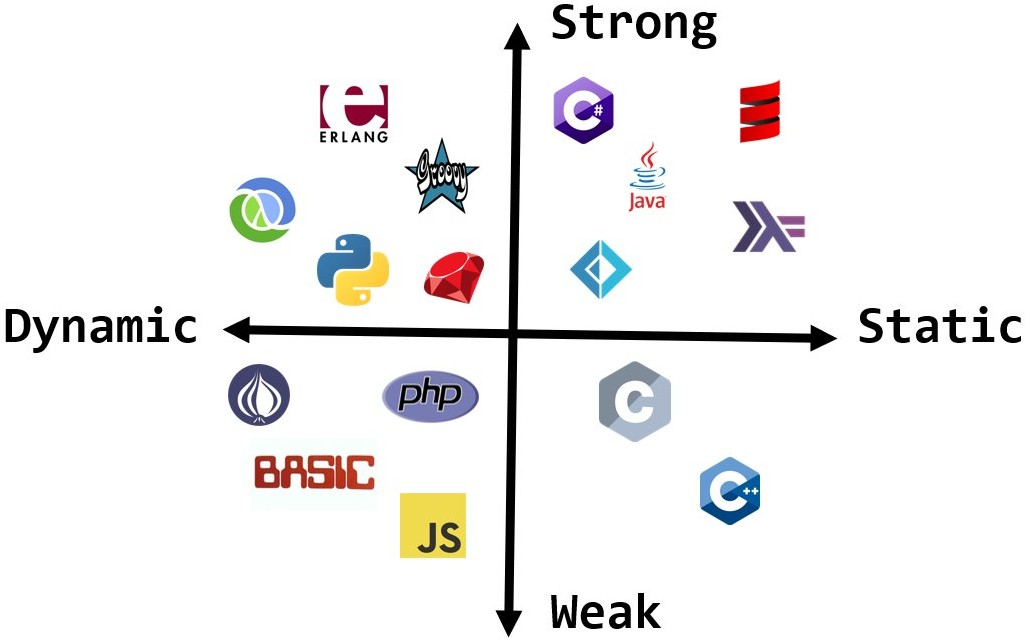
\includegraphics[width=10cm]{types.jpg}\]
\end{frame}

\begin{frame}
	\frametitle{Dynamic vs. Static Programming Languages}
	\[
		{\color{blue}\underline{\href{https://www.online-python.com/}{\text{Demonstration}}}}
	\]
\end{frame}

\begin{frame}
	\frametitle{Where does Formalization come from?}
	\begin{enumerate}
		\item First steps in the 60s and 70s with \textbf{Automath} and \textbf{Logic for Computable Functions} 
		\item In the 80s and 90s, we have the first languages that are still relevant: \textbf{Coq}, \textbf{Isabelle}, \textbf{Agda}, \textbf{PVS}
		\item Since the 2000s: 
		\begin{itemize}
		 \item New languages: \textbf{Metamath}, \textbf{Lean}, ...
		 \item Formalization of interesting problems: \textbf{Four color theorem} (2005), \textbf{Kepler conjecture} (2014), ...
		\end{itemize}
	 \item \textbf{Why now?} User friendlier, AI, ... 
	\end{enumerate}
\end{frame}


\begin{frame}
	\frametitle{Formalization in Programming}
	\begin{figure}
		\centering
		% First row of images
		\begin{subfigure}[b]{0.45\textwidth}
						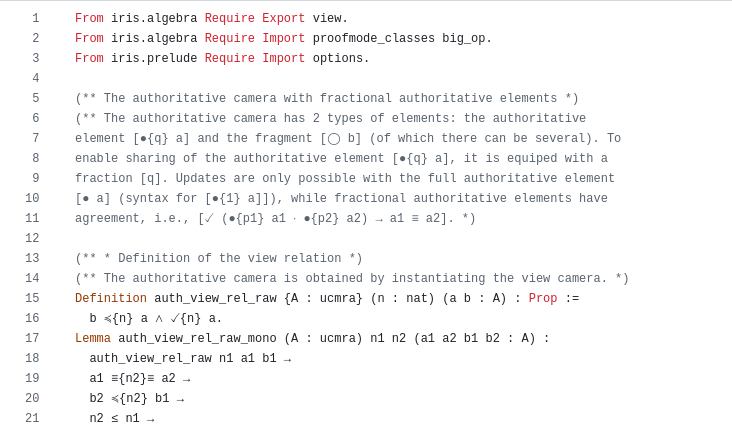
\includegraphics[width=\textwidth]{iris.png}
						\caption{\tiny \textbf{Coq} Iris}
		\end{subfigure}
		\hspace{0.5cm}
		\begin{subfigure}[b]{0.45\textwidth}
						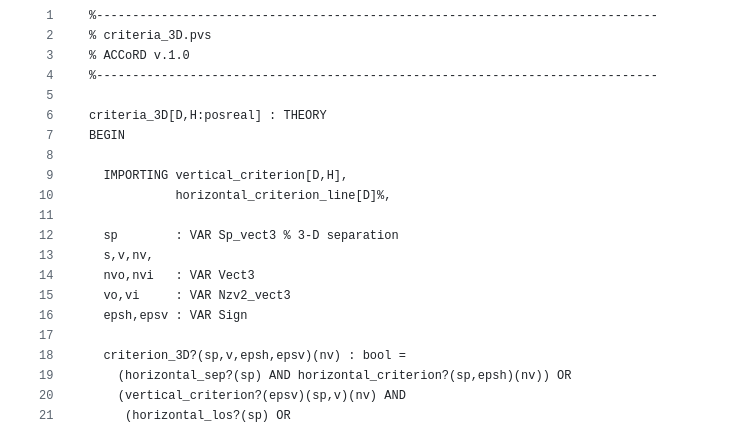
\includegraphics[width=\textwidth]{pvs.png}
						\caption{\tiny \textbf{PVS} in NASA}
		\end{subfigure}

		\vspace{0.2cm} % Space between rows
		% Second row of images
		\begin{subfigure}[b]{0.45\textwidth}
						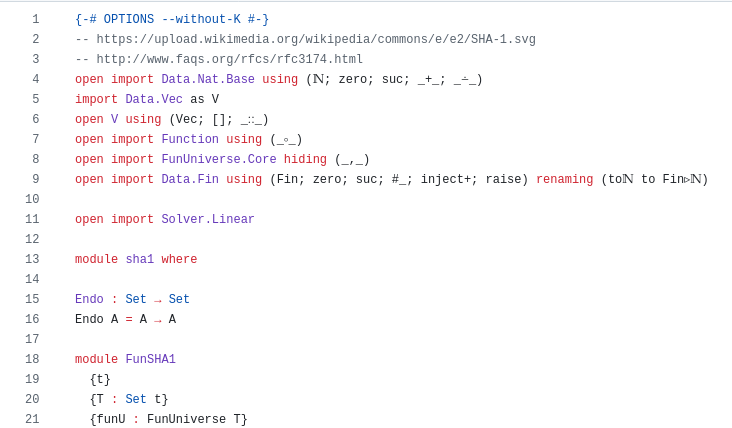
\includegraphics[width=\textwidth]{cryptoagda.png}
						\caption{\tiny \textbf{Agda} in Cryptography $\&$ Blockchain}
		\end{subfigure}
		\hspace{0.5cm}
		\begin{subfigure}[b]{0.45\textwidth}
						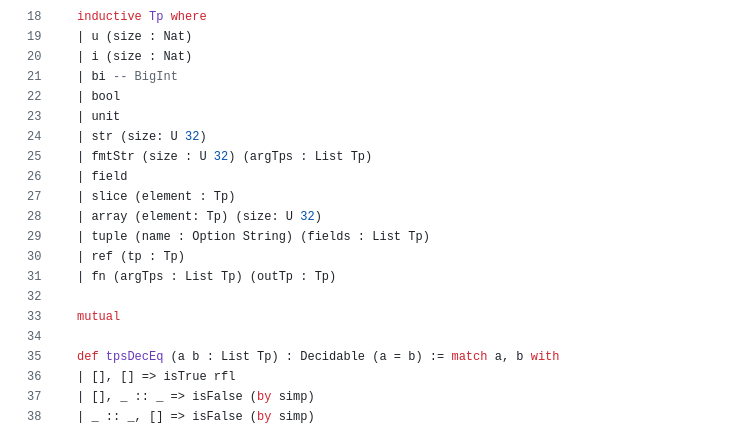
\includegraphics[width=\textwidth]{rust.png}
						\caption{\tiny \textbf{Lean} in Cryptography}
		\end{subfigure}

\end{figure}
\end{frame}

\begin{frame}
	\frametitle{Formalization in Mathematics}
 \begin{figure}
		\centering
		% First row of images
		\begin{subfigure}[b]{0.45\textwidth}
						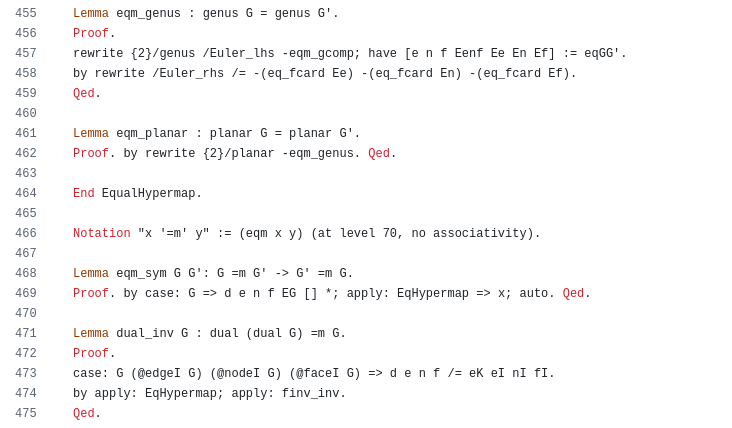
\includegraphics[width=\textwidth]{fourcolor.png}
						\caption{\tiny Four color theorem in \textbf{Coq}}
		\end{subfigure}
		\hspace{0.5cm}
		\begin{subfigure}[b]{0.45\textwidth}
						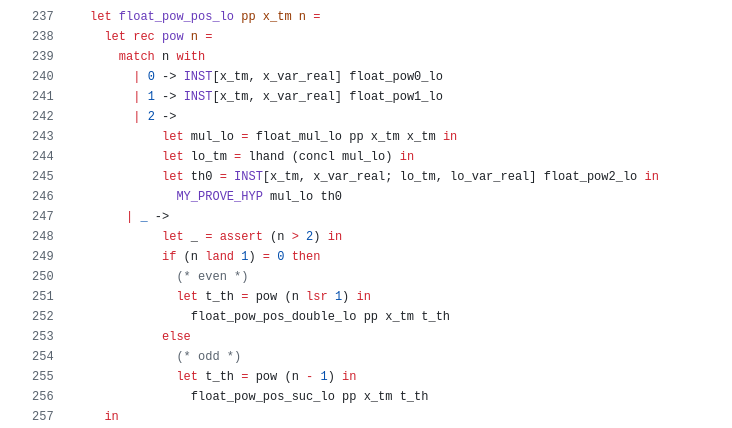
\includegraphics[width=\textwidth]{kepler.png}
						\caption{\tiny Kepler conjecture in \textbf{Isabelle}}
		\end{subfigure}

		\vspace{0.2cm} % Space between rows
		% Second row of images
		\begin{subfigure}[b]{0.45\textwidth}
						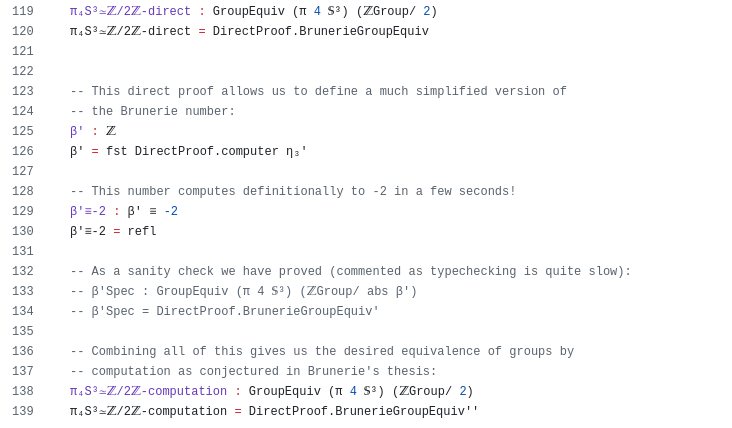
\includegraphics[width=\textwidth]{cubicalagda.png}
						\caption{\tiny Homotopy groups in \textbf{Cubical Agda}}
		\end{subfigure}
		\hspace{0.5cm}
		\begin{subfigure}[b]{0.45\textwidth}
						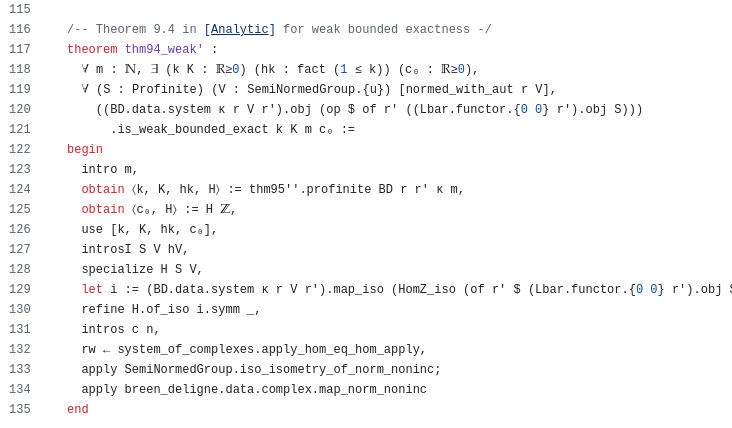
\includegraphics[width=\textwidth]{liquidtensor.png}
						\caption{\tiny Liquid Tensor Experiment in \textbf{Lean}}
		\end{subfigure}
	
\end{figure}
\end{frame}

\begin{frame}
	\frametitle{100 Problems}
	\[
		{\color{blue}\underline{\href{https://www.cs.ru.nl/~freek/100/}{\text{Demonstration}}}}
	\]
\end{frame}

\begin{frame}
	\frametitle{Lean}
		\begin{enumerate}
			\item We use Lean (Lean 4).
			\item Lean is a functional programming language and proof assistant.
			\item Lean was developed in 2013 by Leonardo de Moura (first at Microsoft, now at Amazon).
			\item Lean 4 was released in 2021 and should not change anymore.
			\item Structurally, it resembles Coq. 
			\item Mathematics in Lean is in MathLib Library! 
			\item \textbf{Relatively} easy to use and learn.
			\item But there \textbf{are} many other options!
		\end{enumerate}
\end{frame}

\begin{frame}
	\frametitle{Lean Online}
	
	\[
		{\color{blue}\underline{\href{https://lean-lang.org/}{\text{Demonstration}}}}
	\]
\end{frame}
\begin{frame}
	\frametitle{Logic from a different Perspective}
	\begin{itemize}
		\item In classical mathematics, there is \textbf{Mathematics} and \textbf{Logic}.
		\item \emph{Let} $f\colon S \to T$ \emph{be} a \textbf{bijective} \textbf{function} of \textbf{sets}. \emph{Then} $f$ \emph{is} \textbf{injective}. 
		\item \textbf{Mathematics} vs. \emph{Logic}! \vspace{1cm}
	\end{itemize}
 $\Rightarrow$ We need math and logic in one place!
\end{frame}

\begin{frame}
	\frametitle{Proofs as Elements}
	\[
		{\color{blue}\underline{\href{https://qftx.physik.hu-berlin.de/wp-content/uploads/2012/09/blackboard.jpg}{\text{Demonstration}}}}
	\]
\end{frame}

\begin{frame}
	\frametitle{Examples}
	\[
	\begin{tabular}{|c|c|}
		\hline 
		\textbf{Classical} & \textbf{What we want} \\ \hline
		Prop $P$ & $P :$ Prop \\ 
		Formula for Set X & Function f$\colon$ X $\to$ Prop \\
		Proof for prop $P$ & $\sigma : P$ \\
		Proof for $P \to Q$ & Function $P \to Q$ \\ 
		x = y & (x = y) not empty \\ \hline 
	\end{tabular}
	\]
	Proof for prop 
	\[ \exists S \forall X \forall f,g\colon S \to X (f = g)\]
 \[
	\begin{tabular}{|l|l|} \hline 
		A set S & A pair $(S,\pi)$ \\
		and a proof f = g & $\pi \colon (X,f,g) \to (f = g) $ \\ \hline 
	\end{tabular}
	\]
\end{frame}

\begin{frame}
	\frametitle{Examples in Lean}
	\[
		{\color{blue}\underline{\href{https://pathwaysmiddlecollege.org/wp-content/uploads/2023/11/image.png}{\text{Demonstration}}}}
	\]
\end{frame}

\end{document}
